\chapter{Discussion}

We wish to compare the two-dimensional (2D) GLCM methods to the three-dimensional (3D), to see if one is superior. To make this comparison we have for our data of 100 patients extracted four data sets for left hippocampus. Data set one, D$_1$, we performed erosion before calculating the GLCMs which are normalized, both are done for the 2D and 3D methods. Data set two, D$_2$, is the same as D$_1$ except no erosion has been performed. Data set three, D$_3$, is with erosion, but no normalizing. Data set four, D$_4$, is without erosion and normalizing.
We also wish to determine which of the left or right hippocampus is best suited to diagnose AD, if there is a difference. Data sets D$_5$, D$_6$, D$_7$, D$_8$ are created as D$_{1-4}$ but on the right hippocampus.\\
Lastly we wish to determine if we can correctly diagnose AD with an accuracy higher than 80\%.

In the previous chapter we saw the plots of our data, which are early AD patient, more specific 24-month follow-ups and control. As our data consists of early AD patients, it can be very difficult to differentiate one from another and thus make it challenging to get some good results, specially if we are to select some features to do machine learning. But luckily we can lean on our algorithm to select features better than we can. In consideration of that we have to feature selection method, the first one is naive selection and the second one is Sequential Feature Selection.

\section{Naive feature selection}
As described previously, often there is no clear visual difference in the plots of the GLCM features, which makes it hard to make a naive selections. The way we selected the appropriate data was with us looking at the mean of the data with the respective plot of the respective GLCM.\\
We are only considering 3D eroded and normalized GLCMs for the naive feature selection and chose the following eight features. The Information measures of correlation 2 with the offsets \{(0 -2 2), (0 0 3), (0 -3 0)\} because we can se that generally the control data have a shift down, e.g. the slope is behaving differently than the slope for the AD patients. The next two we elected to our features are information measures of correlation 1 with offsets \{(0 -9 0), (0 -6 6)\} since the AD data seems to have lower values than the control and AD is more spread and has a steep sleep downwards compared to the control. Entropy with the offsets \{(0 -6 6), (0 -10 0)\} is chosen because the AD seems to be more spread and have lower values than control whereas the control is more concentrated in the same spot and the slope seems to be linear for the control. Lastly we have chosen Sum Average with only one offset \{(0 -6 6)\} and this is because it seems that the AD data deviate more than the control.

Considering we only selected eight features we used en exhaustive search to find the optimal model. For each combination of the features we created a KNN model with \emph{k} ranging from one to ten, each models performance was estimated using a 10-fold cross-validation where we randomized the folds 100 times and averaged the accuracy to limit variance. While an exhaustive search is very computational heavy there are only $8! = 40320$ combinations which is nothing compared to the SFS run on the entire feature set.

With our tests we came to the conclusion that we got the best accuracy for only 4 of our 8 features as seen in table \ref{tab:numberOfFeatures}. This table is compares the best accuracy we can get for an unspecific \textit{k} but compares how many features we have to chose out of the 8.

\begin{table}[H]
  \centering
    \begin{tabular}{|c|c|c|c|c|c|c|c|}
    1 Feature  & 2 Features & 3 Features  & 4 Features  & 5 Features  & 6 Features & 7 Features  & 8 Features \\
    \hline
    0.7921  & 0.8166  & 0.8134  & 0.8267  & 0.7924  & 0.7915 & 0.7980  & 0.7981 \\
    \hline
    \end{tabular}%
  \caption{Accuracy for number of features with a unknown k value, we looked after the best accuracy. So this table tells us with how many features how we would get the best accuracy. As seen with only 4 features selected, it has the highest accuracy}\label{tab:numberOfFeatures}%
\end{table}%

The highest accuracy we end up with is 82.67\% for the 4 features selected. As you can see in table \ref{tab:AccuracyTable}, those features are feature 2, 6, 7 and 4 which is equivalent to IMOC2 angle 3 and distance 3, IMOC1 angle 13 and distance 9, Entropy angle 13 and distance 10 and Entropy angle 7 and distance 7. This also suggests that a naive feature selection is not the best, since 50\% of the data will lower the accuracy rather then increase it as we thought it would as seen in table \ref{tab:numberOfFeatures}.

\begin{table}[H]
  \centering
    \begin{tabular}{|c|c|c|c|c|c|c|c|c|c|}
    \hline
               &F 1 &F 2 &F 3 &F 4 &F 5 &F 6 &F 7 &F 8   \\ \hline
             Feature 1&0 &   0.8081 &   0.8173 &        0 &   0.8177 &   0.7959 &        0 &        0 \\
             Feature 2&0 &        0 &   0.8208 &        0 &   0.8145 &   \textbf{0.8267} &        0 &        0 \\
             Feature 3&0 &        0 &        0 &        0 &   0.8114 &   0.7995 &        0 &        0 \\
             Feature 4&0 &        0 &        0 &        0 &        0 &        0 &        0 &        0 \\
             Feature 5&0 &        0 &        0 &        0 &        0 &   0.7938 &        0 &        0 \\
             Feature 6&0 &        0 &        0 &        0 &        0 &        0 &        0 &        0 \\
             Feature 7&0 &        0 &        0 &        0 &        0 &        0 &        0 &        0 \\
             Feature 8&0 &        0 &        0 &        0 &        0 &        0 &        0 &        0 \\ \hline
    \end{tabular}%
  \caption{Where F stands for Feature \#. For feature 7 and feature 4, where it seem that we get the best accuracy with feature 2 and 6. The reason that rows for feature 7 and 4 are zeros is because those features are already selected.}\label{tab:AccuracyTable}%
\end{table}%

It should be noted that there are a few other feature combinations that gives an accuracy of 82.67\%, but this is the first feature combination we run in to were the highest accuracy is 82.67\%

With an algorithm we wish to tell wether we can get a better accuracy or not and for this we use the SFS. As described we have a limit of picking a maximum of 15 features or if the accuracy changes in a negative way. So for every feature to be selected, we choose that which at the given time describes the model with the best accuracy and this means that we can end up with \texttt{n} features but a maximum of 15.\\
For the 2D SFS have a feature accuracy of 91\% for $k=3$ as seen in table \ref{tab:Features2d3k}

\begin{table}[htbp]
  \centering
    \begin{tabular}{|r|r|r|r|r|}
    \hline
          & Feature Accuracy & Offset & Metric & Distance \\
    \hline
    Feature 1 & 0.81  & 4     & 8     & 7 \\
    \hline
    Feature 2 & 0.87  & 2     & 13    & 7 \\
    \hline
    Feature 3 & 0.89  & 8     & 1     & 3 \\
    \hline
    Feature 4 & 0.9   & 8     & 13    & 8 \\
    \hline
    Feature 5 & 0.91  & 2     & 1     & 7 \\
    \hline
    Feature 6 & 0.91  & 4     & 13    & 7 \\
    \hline
    \end{tabular}%
    \caption{Six features shown for $k=3$}\label{tab:Features2d3k}%
\end{table}%

This means that we have a feature accuracy of 91\% with only 5 features, but it is still interesting to see how well the model can predict the data with these features

\begin{figure}[H]
  \centering
  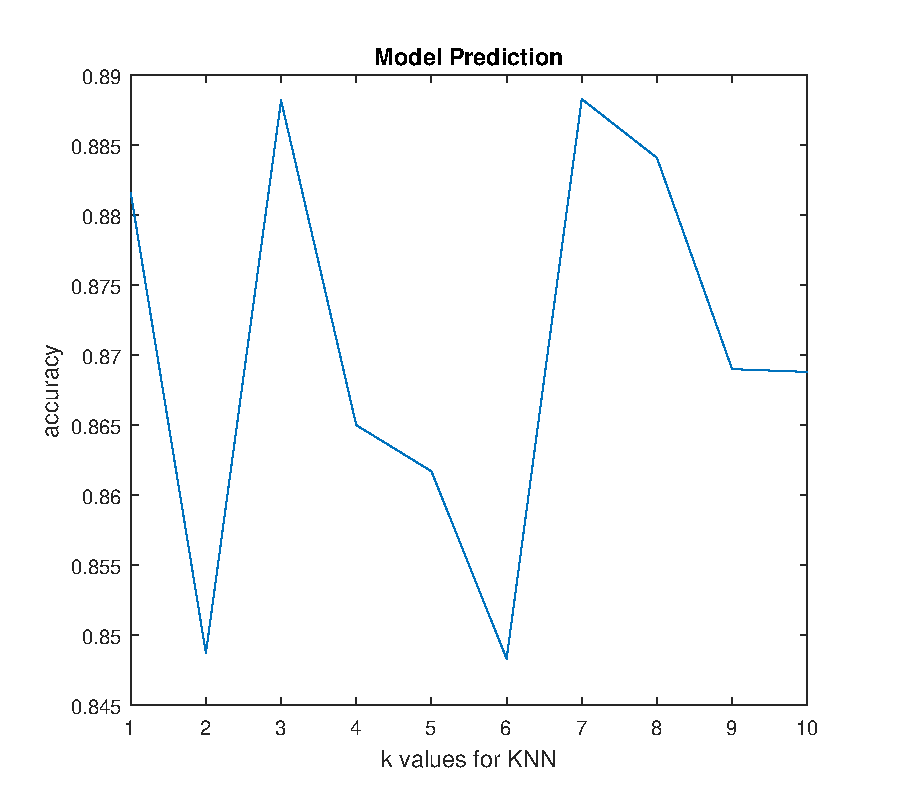
\includegraphics[scale=0.65]{acc2D3k.eps}
  \caption{Plot of the accuracy for the 2D of our model with a feature accuracy of 91\% and model accuracy with k values from 1 to 10 for KNN}\label{fig:Features2d3k}
\end{figure}

It should be noted that there is a possibility that for $k=3$ the model could be biased because we have chosen features for $k=3$ as seen in table \ref{tab:Features2d3k}. As seen in figure \ref{fig:Features2d3k} the model has the highest accuracy for both $k=3$ and $k=7$ which means that for nearest neighbours 3 and 7 we get of 88.83\% which is slightly higher than the naive feature selection, but it should be noted the this is done for 2D and the naive is 3D. So lets compare the 3D SFS with the naive selection which is more fair.

With the 3D SFS it seems that $k=1$ is in favor with the highest feature accuracy as seen in tab \ref{tab:Features3d1k} with a whole of 10 features before the feature accuracy does not improve any more

\begin{table}[H]
  \centering
    \begin{tabular}{|r|r|r|r|r|}
    \hline
          & Accuracy & Offset & Metric & Distance \\
    \hline
    Feature 1 & 0.82  & 10    & 13    & 2 \\
    \hline
    Feature 2 & 0.86  & 4     & 13    & 5 \\
    \hline
    Feature 3 & 0.87  & 12    & 13    & 7 \\
    \hline
    Feature 4 & 0.87  & 12    & 8     & 7 \\
    \hline
    Feature 5 & 0.87  & 5     & 8     & 8 \\
    \hline
    Feature 6 & 0.88  & 10    & 8     & 7 \\
    \hline
    Feature 7 & 0.92  & 2     & 13    & 6 \\
    \hline
    Feature 8 & 0.93  & 6     & 8     & 10 \\
    \hline
    Feature 9 & 0.94  & 8     & 13    & 7 \\
    \hline
    Feature 10 & 0.95  & 3     & 10    & 7 \\
    \hline
    Feature 11 & 0.95  & 4     & 1     & 3 \\
    \hline
    \end{tabular}%
  \caption{Eleven features shown for $k=1$}\label{tab:Features3d1k}%
\end{table}%

With are feature accuracy of 95\% with 10 features needed, we are now interested to see what the model can predict.

\begin{figure}[H]
  \centering
  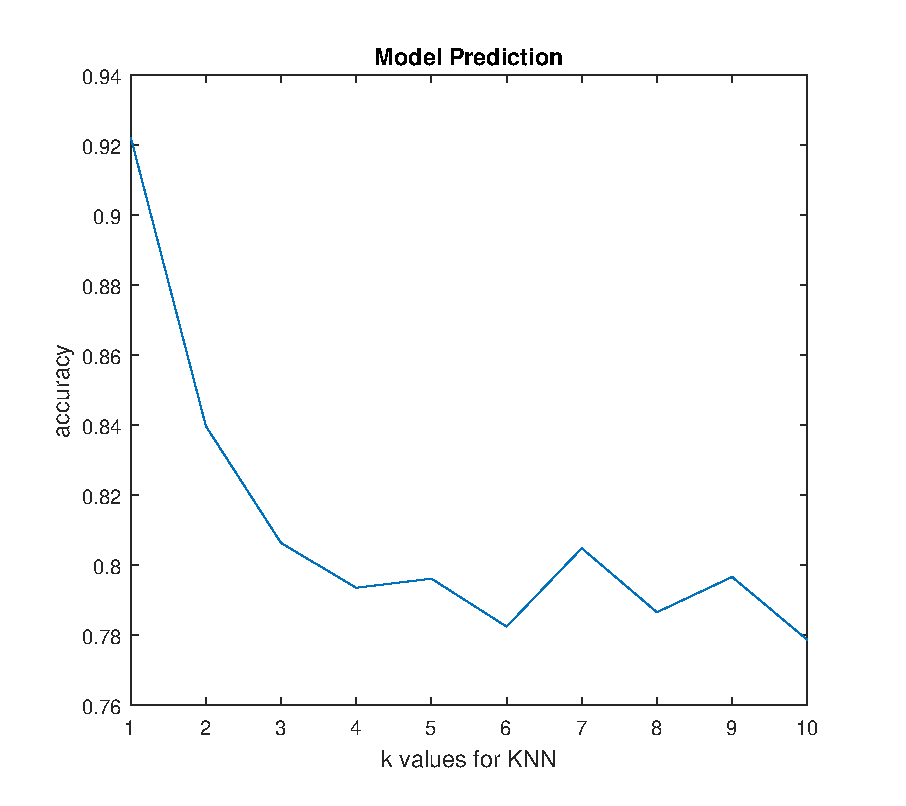
\includegraphics[scale=0.65]{acc3D1k.eps}
  \caption{Plot of the accuracy for the 3D of our model with a feature accuracy of 95\% and model accuracy with k values from 1 to 10 for KNN}\label{fig:Features3d1k}
\end{figure}

As it is possible to see in figure \ref{fig:Features3d1k} the accuracy is 92.23\% for $k=1$, which can be biased. This accuracy is also a lot higher than what we got with the naive feature selection. It is shown in figure \ref{fig:Features3d1k} that when we expand our search to more than 1 nearest neighbour that the accuracy falls drastically.

It was possible to get an accuracy higher than the desired 80\% for even a feature selection as simplistic as the naive.

\section{Comparison of image textures}
For each of the methods, and for each data set we have run a feature selection and fitted a model the features selected for each model. For the 3D model on D$_4$ there was a tie between two different \emph{k}, and the accuracy for both models were calculated.

\begin{table}[H]
  \centering
    \begin{tabular}{|r|r|r|r|r|}
    \hline
    K     & 2DLNE & 2DLE  & 2DLN  & 2DL \\ \hline
    1     & 0,8816 & \textbf{0,9203} & 0,8441 & \textbf{0,9255} \\ \hline
    2     & 0,8487 & 0,8511 & 0,8688 & 0,9186 \\ \hline
    3     & 0,8882 & 0,8641 & 0,8837 & 0,875 \\ \hline
    4     & 0,865 & 0,8351 & 0,8878 & 0,8376 \\ \hline
    5     & 0,8617 & 0,8011 & \textbf{0,8997} & 0,8385 \\ \hline
    6     & 0,8483 & 0,8003 & 0,8712 & 0,8317 \\ \hline
    7     & \textbf{0,8883} & 0,7975 & 0,8713 & 0,8187 \\ \hline
    8     & 0,8841 & 0,7945 & 0,8751 & 0,8286 \\ \hline
    9     & 0,869 & 0,7938 & 0,869 & 0,8249 \\ \hline
    10    & 0,8688 & 0,783 & 0,8496 & 0,8266 \\ \hline
    \end{tabular}%
  \caption{2D: Accuracy of final KNN-model L = left, E = erosion, N = normalized}\label{tab:2DFinalModel}%
\end{table}%

Interestingly for the the 2D method is the best accuracies occur when the data is not normalized, suggesting that there is a significant difference in the amount GI's between the two groups. There is also a substantial drop in accuracy with increased \emph{k} value for the KNN, further validating that the size difference between the groups is relevant. This is in stark contrast to the normalized data, as they do not vary a lot between the \emph{k}'s, there is some peaks though.\\
There is no clear difference between the eroded and non eroded models. We erode the image with a three-dimensional model, so it is possible that the offsets in the 2D model does not get the benefit of this erosion. It could also be that the original segmentation is done very well and erosion is not necessary for these images. It does not decrease performance either, so it does not suggest relevant data is lost.

\begin{table}[H]
  \centering
    \begin{tabular}{|r|r|r|r|r|r|}
    \hline
    K     & 3DLNE & 3DLE  & 3DLN  & 3DLk1 & 3DLk3 \\ \hline
    1     & \textbf{0,9223} & 0,8561 & 0,8374 & \textbf{0,8892} & \textbf{0,8436} \\ \hline
    2     & 0,8397 & \textbf{0,8954} & 0,7977 & 0,8072 & 0,8034 \\ \hline
    3     & 0,8063 & 0,8199 & \textbf{0,8914} & 0,8261 & 0,8426 \\ \hline
    4     & 0,7935 & 0,7828 & 0,8191 & 0,7697 & 0,763 \\ \hline
    5     & 0,7961 & 0,7617 & 0,8041 & 0,7626 & 0,7295 \\ \hline
    6     & 0,7824 & 0,7717 & 0,8002 & 0,7299 & 0,704 \\ \hline
    7     & 0,8048 & 0,7714 & 0,7712 & 0,7077 & 0,6922 \\ \hline
    8     & 0,7865 & 0,7777 & 0,7875 & 0,7193 & 0,7121 \\ \hline
    9     & 0,7966 & 0,7808 & 0,7795 & 0,7294 & 0,7152 \\ \hline
    10    & 0,7786 & 0,793 & 0,78  & 0,7524 & 0,7371 \\ \hline
    \end{tabular}%
  \caption{3D: Accuracy of final KNN-model, two values for 3DL since feature selection resulted in a tie between k = 1 and k = 3}\label{tab:3DFinalModel}%
\end{table}%

The poor performance of \emph{3Dlk3} compared to \emph{3DLk1} suggest that the feature selection overfit the data to its specific sample, as in that separation into 10-folds is biased toward a k = 3 for its solution. It also shows that k = 1 is most likely the best KNN model for that data set, as even though \emph{3DLk3} is biased toward k = 3, it performs equally well for k = 1, where as \emph{3DLk1} is clearly performs better for k = 1 opposed to k = 3. All the models best \emph{k} value is also equal to the \emph{k} returned from their feature selection, highlighting the overfitting towards that specific model done in the feature selection.\\
For the normalized data the model created on the data set with erosion perform better than without erosion, but there is no difference on the data that is not normalized. On the data sets that is not normalized the number of observations is a relevant factor, then it is not unrealistic that the erosion removes a similar percentage of data from both control and AD, thus not being creating a difference between a model using erosion and one that does not, and would only impact their overall accuracy if there is a lot of noise in the border region of the segmentation. But as we saw in the 2D method, where erosion did not play a significant role in accuracy it is not clear it is does for the 3D method either.

The top accuracies for the 2D methods is 92.0\% and 92.5\% and for the 3D methods it is 92.2\% which makes it very hard to declare a winner, also considering that the rest of the predictions is just below 90\% the methods returns very similar results. However overfitting appears to be more prevalent in the feature selection in the 3D methods, as can be seen by the rapidly deteriorating accuracy when \emph{k} diverges from the optimal \emph{k} used to select the features. The reason for the overfitting will be discussed later.

The difference in methods between 2D and 3D are only four offsets, so if method based in 3D is to be superior to a 2D one the four additional angles would need to contain information describing the inter-relations between voxels better. The four offsets are \{(d, -d, -d), (-d,-d,-d), (-d, -d, d), (d, -d, d)\} which translates into no. \{6,8,10,12\} and when we look at the features selected by the 3D methods we notice they are being used, but not exclusively.
\begin{table}[H]
  \centering
    \begin{tabular}{|c|c|c|c|}
    \hline
    3DL F & Offset & Feature & Distance \\ \hline
    Feature 1 & 12    & 4     & 1 \\ \hline
    Feature 2 & 4     & 5     & 10 \\ \hline
    Feature 3 & 5     & 9     & 9 \\ \hline
    Feature 4 & 4     & 8     & 10 \\ \hline
    \end{tabular}%
 \caption{Feature selected for 3D no erosion,without normalization}\label{tab:3DL F}%
\end{table}%
\begin{table}[H]
  \centering
    \begin{tabular}{|c|c|c|c|}
     \hline
    3DLN F & Offset & Feature & Distance \\ \hline
    Feature 1 & 6     & 12    & 3 \\ \hline
    Feature 2 & 5     & 11    & 7 \\ \hline
    Feature 3 & 4     & 11    & 10 \\ \hline
    Feature 4 & 4     & 8     & 10 \\ \hline
    \end{tabular}%
 \caption{Feature selected for 3D no erosion, with normalization}\label{tab:3DLN F}%
\end{table}%


\begin{table}[H]
  \centering
    \begin{tabular}{|c|c|c|c|}
     \hline
            3DLE F & Offset & Feature & Distance \\ \hline
          Feature 1& 5     & 8     & 3 \\ \hline
          Feature 2& 3     & 8     & 1 \\ \hline
          Feature 3& 1     & 9     & 4 \\ \hline
          Feature 4& 2     & 10    & 1 \\ \hline
          Feature 5& 11    & 7     & 7 \\ \hline
          Feature 6& 12    & 11    & 5 \\ \hline
          Feature 7& 8     & 8     & 10 \\ \hline
          Feature 8& 5     & 7     & 3 \\ \hline
          Feature 9& 2     & 7     & 3 \\ \hline
          Feature 10& 12    & 7     & 4 \\ \hline
          Feature 11& 1     & 7     & 4 \\ \hline
          Feature 12& 4     & 7     & 5 \\ \hline
          Feature 13& 8     & 7     & 6 \\ \hline
    \end{tabular}%
  \caption{Feature selected for 3D with erosion, without normalization}\label{tab:3DEnorm}%
\end{table}%


\begin{table}[H]
  \centering
    \begin{tabular}{|c|c|c|c|}
     \hline
    3DLNE F & Offset & Feature & Distance \\ \hline
        Feature 1& 10    & 13    & 2 \\ \hline
        Feature 2& 4     & 13    & 5 \\ \hline
        Feature 3& 12    & 13    & 7 \\ \hline
        Feature 4& 12    & 8     & 7 \\ \hline
        Feature 5& 5     & 8     & 8 \\ \hline
        Feature 6& 10    & 8     & 7 \\ \hline
        Feature 7& 2     & 13    & 6 \\ \hline
        Feature 8& 6     & 8     & 10 \\ \hline
        Feature 9& 8     & 13    & 7 \\ \hline
    \end{tabular}%
  \caption{Features selected for 3D erosion and normalization}\label{tab:3DLNE}%
\end{table}%

The first two tables, \ref{tab:3DL F} and \ref{tab:3DLN F}, only use one out of four, the third table \ref{tab:3DEnorm} use four out of thirteen, and the last table \ref{tab:3DLNE} use six out of nine, totalling to twelve out of thirty which is equal to 40\%. They compromise four out of thirteen of the offsets which is $\approx$ 30\% so they are over represented, suggesting they do contain better data than the original offsets. They are also selected as the first feature in three tables \{\ref{tab:3DL F},\ref{tab:3DLN F},\ref{tab:3DLNE}\} of the four feature selections, meaning the single best feature is found three times out of four in one of the offsets unique to the 3D methods. Which are very promising regarding the 3D methods but considering the accuracy they do not despite these additional offsets outperform the 2D methods, and with four more offsets they have an additional $4\cdot13\cdot10 = 520$ features compared to the 2D. Most of the selected models only use a number of features between 4 and 13 which is less than 0.1\% of the total number of features, the additional offsets only increases computational time notably without any significant benefit.
\begin{table}[H]
    \centering
    \begin{tabular}{|r|r|r|r|r|r|}
    \hline
    2D    & 92    & 89    & 92    & 96    & 93 \\ \hline
    3D    & 129   & 128   & 127   & 134   & 132 \\ \hline
    ratio & 1,402 & 1,438 & 1,380 & 1,400 & 1,419 \\ \hline
    2D    & 125   & 125   & 127   & 121   & 118 \\ \hline
    3D    & 176   & 178   & 175   & 171   & 170 \\ \hline
    ratio & 1,408 & 1,424 & 1,378 & 1,413 & 1,440 \\ \hline
    \end{tabular}%
    \caption{Run time in seconds to select a single feature in 2D vs 3D, calculated on two different machines}\label{tab:Time}%
\end{table}%
As we can see in table \ref{tab:Time} the 3D feature selection takes $\approx$40\% longer to select a single feature. The added computational cost of adding additional offsets suggest that one should look elsewhere to improve the accuracy. Considering that not normalizing the data gives comparable and even superior results in 2D would suggest that creating new features closer related to the number of elements in the GLCMs would improve results, but that is beyond the scope of this paper.

Considering the similar accuracy of the 2D and 3D methods, we recommend using a 2D method as it has significant faster run time, without any decrease in accuracy. It is also worth noting that it is indeed possible to predict AD with an accuracy of above 80\%, event if we were to use a different \emph{k} value than the one that is optimal from the feature selection. Especially the 2D methods that included normalization produced models that predicted in the mid eighties, for all \emph{k} in one to ten.

\section{Hippocampus comparison}

The method used on the right is the same as on the left, however the accuracies are not of similar quality, as can be seen in table \ref{tab:RightModels}.
\begin{table}[H]
  \centering
    \begin{tabular}{|r|r|r|r|r|r|r|r|r|}
     \hline
    K     & 3DRNE & 3DRN  & 3DRE  & 3DR   & 2DRNE & 2DRN  & 2DRE  & 2DR \\  \hline
    1     & <.80  & <.80  & 0,8194 & <.80  & \textbf{0,8326} & <.80  & <.80  & <.80 \\  \hline
    2     & \textbf{0,8514} & <.80  & \textbf{0,8746} & <.80  & <.80  & \textbf{0,8891} & <.80  & 0,8157 \\ \hline
    3     & <.80  & <.80  & <.80  & <.80  & <.80  & 0,8668 & <.80  & 0,8624 \\ \hline
    4     & <.80  & <.80  & <.80  & 0,8398 & <.80  & 0,8883 & 0,8459 & \textbf{0,8992} \\ \hline
    5     & <.80  & <.80  & <.80  & 0,8312 & <.80  & 0,8391 & 0,8337 & <.80 \\ \hline
    6     & <.80  & <.80  & <.80  & \textbf{0,8413 }& <.80  & 0,8455 & 0,8486 & <.80 \\ \hline
    7     & <.80  & <.80  & <.80  & <.80  & <.80  & <.80  & 0,8495 & <.80 \\ \hline
    8     & <.80  & <.80  & <.80  & <.80  & <.80  & <.80  & \textbf{0,8730} & <.80 \\ \hline
    9     & <.80  & <.80  & <.80  & <.80  & <.80  & <.80  & 0,8475 & <.80 \\ \hline
    10    & <.80  & <.80  & <.80  & <.80  & <.80  & <.80  & 0,852 & <.80 \\ \hline
    \end{tabular}%
    \caption{Accuracy of models calculated on the right hippocampus}\label{tab:RightModels}%
\end{table}%
Especially the 3D model does not give great results except for the method with only erosion which have a 87\% accuracy, but that compared to the accuracy for the left seen in table \ref{tab:3DFinalModel} with 89.5\% it is still lacking behind. That is the general picture for all methods.\\
From the beginning we made all calculation using the left hippocampus data as test on the functions to validate they work as intended. First when we were done with the entire model, did we apply it on the right hippocampus, which could introduce bias towards the left hippocampus data.

\section{Overfitting}
In the forward feature selection algorithm we attempt to avoid overfitting by creating a 10-fold cross validation, but in order to avoid overfitting more successfully it would be a better idea to keep randomizing the folds, our implementation creates the folds firstly and then run the entire feature selection without shuffling the folds. Since we do not reshuffle the data we are making our feature selection biased towards this specific partition. We can see this bias by running a test using our forward feature selection on 60 patients, and using the last 40 to test. In addition to only running one cross-validation we do not minimize the effect of its variance which can potentially lead to poor choices. Considering we evaluate all features with the cross-validation it is most likely that some of get a higher evaluation due to the variance.\\
Running the feature selection on the data gained from using three-dimensional GLCMs with erosion and normalizing, and using 10-fold cross validation, with 6 (3 Control and 3 AD) in each folds. The feature selection results in an accuracy of 98\% on KNN model, with k = 1. However testing this model on the remaining 40 patients using 10-fold cross validation with 4(2 Control and 2 AD) in each fold, the accuracy is instead 80\% and the best k value for the KNN model is instead  k = 3 or k = 5.\\
Running the same test on the two-dimensional we get an accuracy of 95\% with optimal k = 1 or k = 3, where each k does not select the same features but do have some overlap. The model created using the features from the first k gives us an accuracy of 82.50\% when validating with the test set and optimal k = 9, the other model has an accuracy of 80\%, obtained for each of k ={2,3,5,7}. This does not account for the variance in the cross-validation, so by running the cross-validation 100 times we get an accuracy of 80\% for k = 1, suggesting that our feature selection overfit in its estimation.\\
This overfitting could have been countered by running more than one 10-fold cross-validation when estimating the features predictability. If we had used the same cross-validation we use to evaluate the final models, the feature selection would not return accuracies in the 95+\%, but it would still be biased towards the k it is selected for. To avoid bias towards the specific \emph{k} value we would have needed a different evaluation criterion instead of the KNN we currently use.

